\documentclass[11pt]{article}
\usepackage[margin=1in]{geometry}
\usepackage{amsmath,amssymb}
\usepackage{graphicx}
\usepackage{xcolor}
\usepackage{tikz}
\usetikzlibrary{decorations.pathmorphing,decorations.pathreplacing,arrows.meta,calc}
\usepackage{pgfplots}
\pgfplotsset{compat=1.17}
\usepackage{tcolorbox}
\usepackage{booktabs}
\usepackage{array}
\usepackage{enumitem}
\usepackage{hyperref}

\graphicspath{{figures/}}

% Notation
\newcommand{\xs}{x_{\text{stim}}}
\newcommand{\xd}{x_{\text{dist}}}
\newcommand{\xp}{x_{\text{perc}}}
\newcommand{\PSEuni}{\mathrm{PSE}_{\text{uni}}}
\newcommand{\PSEbi}{\mathrm{PSE}_{\text{bi}}}
\newcommand{\high}{\text{``high''}}
\newcommand{\low}{\text{``low''}}

\definecolor{unicol}{RGB}{0,120,230}
\definecolor{bicol}{RGB}{205,0,0}

% Red margin-style notes from the handwritten slides
\newtcolorbox{aside}{colback=red!4,colframe=red!60!black,boxrule=0.5pt,
  left=4pt,right=4pt,top=2pt,bottom=2pt,fontupper=\small,
  title={\small Note},fonttitle=\bfseries\small,coltitle=white}
\newtcolorbox{result}{colback=green!6,colframe=green!45!black,boxrule=0.6pt}

% Trial timeline diagram: #1 = 1 if standard is crossed out, #2 = distractor position (std/cmp)
\newcommand{\timeline}[2]{%
\begin{tikzpicture}[x=1cm,y=1cm,font=\small]
  \node[anchor=east] at (0,1.2) {attended hand};
  \node[anchor=east] at (0,0) {ignored hand};
  \draw[thick] (0.2,1.2) -- (1.2,1.2);
  \draw[thick] (1.2,0.75) rectangle (3.6,1.65);
  \node[align=center] at (2.4,1.2) {standard\\[-2pt]{\footnotesize(fixed)}};
  \draw[thick] (3.6,1.2) -- (4.6,1.2);
  \draw[thick] (4.6,0.75) rectangle (7.0,1.65);
  \node[align=center] at (5.8,1.2) {comparison\\[-2pt]{\footnotesize(varied)}};
  \draw[thick] (7.0,1.2) -- (8.0,1.2);
  \ifnum#1=1
    \draw[red,thick] (1.1,0.65) -- (3.7,1.75);
    \draw[red,thick] (1.1,1.75) -- (3.7,0.65);
  \fi
  \ifnum#2=0
    \draw[thick] (0.2,0) -- (1.2,0);
    \draw[thick,dashed] (1.2,-0.4) rectangle (3.6,0.4);
    \node at (2.4,0) {distractor};
    \draw[thick] (3.6,0) -- (8.0,0);
  \else
    \draw[thick] (0.2,0) -- (4.6,0);
    \draw[thick,dashed] (4.6,-0.4) rectangle (7.0,0.4);
    \node at (5.8,0) {distractor};
    \draw[thick] (7.0,0) -- (8.0,0);
  \fi
\end{tikzpicture}}

\title{Lab Update: Modeling Bimanual Perceptual Interactions in Monkeys}
\author{Vera Schroeder}
\date{January 8, 2026\\[4pt]\small(typeset from handwritten notes for reference)}

\begin{document}
\maketitle
\tableofcontents
\newpage

%=====================================================================
\section{Experimental design: 2AFC task}

\begin{itemize}
  \item \textbf{Stimulus} $\xs \in \{6,\dots,50\}$\textsuperscript{*}
  \begin{itemize}
    \item administered to one hand
  \end{itemize}
  \item \textbf{Distractor} $\xd \in \{0, d\}$\textsuperscript{*}
  \begin{itemize}
    \item $d \in [6,32]$, value fixed per session
    \item administered to the other (non-stimulus) hand
  \end{itemize}
  \item Stimulus and distractor are administered simultaneously.
  \item \textbf{Response choices}
  \begin{itemize}
    \item \low: correct for $\xs \in \{6,12,18,24\}$
    \item \high: correct for $\xs \in \{32,38,44,50\}$
  \end{itemize}
  \item Correct responses are rewarded.
\end{itemize}
\noindent\textsuperscript{*}Amplitude of vibration in microns.

\medskip
The distractor items (and the fact that stimulus and distractor are simultaneous)
are the parts of the design that matter for \emph{modeling bimanual interactions}.

%=====================================================================
\section{Psychometric function}

\begin{center}
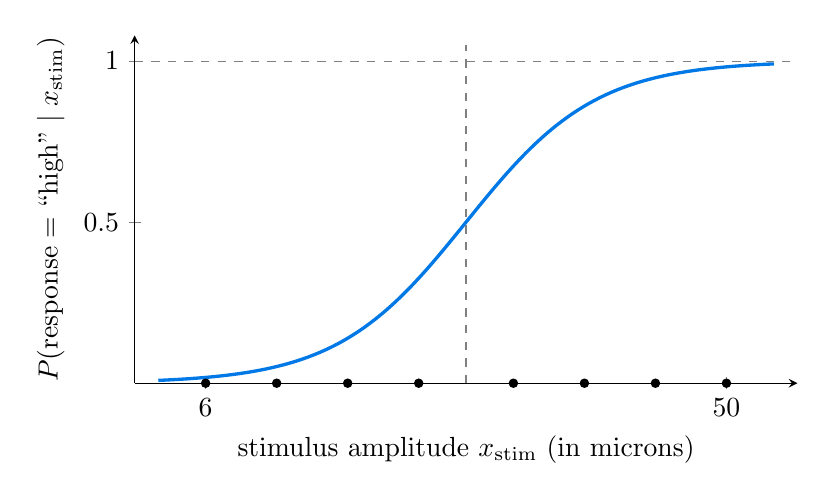
\begin{tikzpicture}
\begin{axis}[width=10cm,height=6cm,
  xmin=0,xmax=56,ymin=0,ymax=1.08,
  xtick={6,50},ytick={0.5,1},
  xlabel={stimulus amplitude $\xs$ (in microns)},
  ylabel={$P(\text{response}=\high \mid \xs)$},
  axis lines=left,clip=false]
  \addplot[domain=2:54,samples=100,very thick,unicol]{1/(1+exp(-(x-28)/5.5))};
  \addplot[only marks,mark=*,mark size=1.5pt] coordinates{(6,0)(12,0)(18,0)(24,0)(32,0)(38,0)(44,0)(50,0)};
  \draw[dashed,gray] (axis cs:0,1) -- (axis cs:56,1);
  \draw[dashed,gray] (axis cs:28,0) -- (axis cs:28,1.05);
\end{axis}
\end{tikzpicture}
\end{center}
\[
  \psi(x;\beta_0,\beta_1) = \frac{1}{1+\exp\bigl[-(\beta_0+\beta_1 x)\bigr]}
\]

%=====================================================================
\section{Incorporating distractor strength into the model}

\textbf{Hypothesis.} The amplitude perceived on the stimulated hand is a combination
of the signals received by both hands, with the weight of the distractor decreasing
over sessions with fixed distractor difficulty:
\[
  \xp = \xs + \varepsilon_{\text{noise}} + c\,\bigl(\xd + \varepsilon_d\bigr),
  \qquad \varepsilon_{\text{noise}} \sim \operatorname{Logistic}[\mu,\sigma].
\]

\begin{aside}
Try: extra noise is only present in bimanual trials.
\end{aside}

\begin{center}
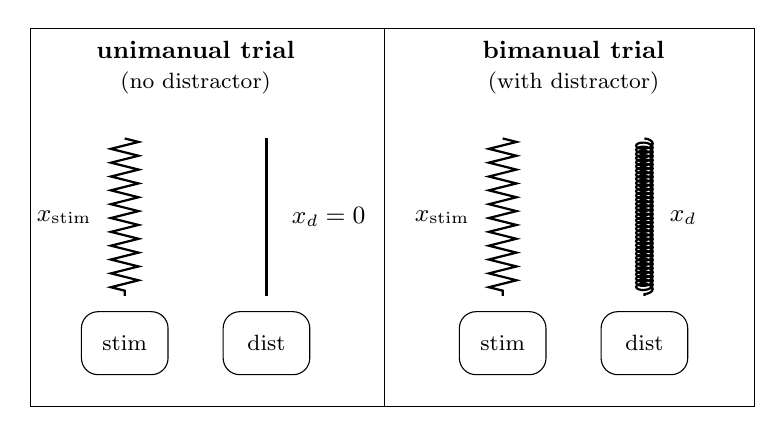
\begin{tikzpicture}[font=\small,
  spring/.style={decorate,decoration={zigzag,segment length=5pt,amplitude=5pt},thick},
  tight/.style={decorate,decoration={coil,segment length=1.5pt,amplitude=3pt},thick},
  hand/.style={draw,rounded corners=6pt,minimum width=1.1cm,minimum height=0.8cm,font=\footnotesize}]
  % unimanual
  \node[align=center] at (1.5,4.3) {\textbf{unimanual trial}\\{\footnotesize(no distractor)}};
  \draw[spring] (0.6,3.4) -- (0.6,1.4); \node[anchor=east] at (0.3,2.4) {$\xs$};
  \draw[thick] (2.4,3.4) -- (2.4,1.4); \node[anchor=west] at (2.6,2.4) {$x_d=0$};
  \node[hand] at (0.6,0.8) {stim};
  \node[hand] at (2.4,0.8) {dist};
  \draw (3.9,0) -- (3.9,4.8);
  % bimanual
  \node[align=center] at (6.3,4.3) {\textbf{bimanual trial}\\{\footnotesize(with distractor)}};
  \draw[spring] (5.4,3.4) -- (5.4,1.4); \node[anchor=east] at (5.1,2.4) {$\xs$};
  \draw[tight] (7.2,3.4) -- (7.2,1.4); \node[anchor=west] at (7.4,2.4) {$x_d$};
  \node[hand] at (5.4,0.8) {stim};
  \node[hand] at (7.2,0.8) {dist};
  \draw (-0.6,0) rectangle (8.6,4.8);
\end{tikzpicture}
\end{center}

%=====================================================================
\section{Psychometric function with a distractor}

\begin{align*}
  \psi(\xs,\xd) &= P\bigl(\high \mid \xs = x_s,\ \xd = x_d\bigr)
  = \frac{1}{1+\exp\bigl[-(\beta_0+\beta_1 x_s+\beta_2 x_d)\bigr]}.
\end{align*}
The linear predictor can be rewritten as
\begin{align*}
  \beta_0+\beta_1\xs+\beta_2\xd
  &= \beta_0+\beta_1\Bigl(\xs+\frac{\beta_2}{\beta_1}\xd\Bigr)\\
  &= \beta_0+\beta_1\underbrace{\bigl(\xs+c\,\xd\bigr)}_{\xp},
  \qquad c = \beta_2/\beta_1 .
\end{align*}

%=====================================================================
\section{Equivalent formulation of $\psi$ (bimanual)}

For a model of bimanual interactions, consider
\[
  \xp = \xs + c\,\xd + \varepsilon, \qquad \varepsilon \sim \operatorname{Logistic}[\mu,s],
\]
and let the decision rule on $\xp$ be
\[
  \text{response} =
  \begin{cases}
    \high, & \text{if } \xp > t,\\
    \low,  & \text{if } \xp < t.
  \end{cases}
\]

\begin{aside}
Why would I set only one threshold instead of using a different one when I know
I'm being distracted?
\end{aside}

Now consider
\begin{align*}
  \psi = P(\text{response}=\high \mid \xs,\xd)
  &= P(\xp > t \mid \xs = x_s,\ \xd = x_d)\\
  &= P(x_s + c x_d + \varepsilon > t)\\
  &= P(\varepsilon > t - x_s - c x_d)\\
  &= 1 - P(\varepsilon < t - x_s - c x_d)\\
  &= 1 - \frac{1}{1+\exp\Bigl[-\Bigl(\dfrac{(t-x_s-c x_d)-\mu}{s}\Bigr)\Bigr]}\\
  &= \boxed{\frac{1}{1+\exp\Bigl[\dfrac{t-x_s-c x_d-\mu}{s}\Bigr]}}\\
  &= \frac{1}{1+\exp\Bigl[-\Bigl(\dfrac{\mu-t}{s}+\dfrac{1}{s}x_s+\dfrac{c}{s}x_d\Bigr)\Bigr]}\\
  &\;:=\; \frac{1}{1+\exp\bigl[-(\beta_0+\beta_1 x_s+\beta_2 x_d)\bigr]}.
\end{align*}
This is equivalent to the previous construction of $\psi$ when
\[
  \beta_0 = \frac{\mu-t}{s},\qquad \beta_1 = \frac{1}{s},\qquad \beta_2 = \frac{c}{s}.
\]
(In the handwritten boxed line, $\mu$ is overwritten with $0$; see the identifiability
remark below.)

\begin{aside}
Follow-up paper: Wichmann \& Hill, statistical inference of psychometric functions
(``weird noise dist.''), noted as ``Psychology Review''.
\end{aside}

\subsection*{At what value of $\xs$ are responses \high{} and \low{} equally likely?}

\begin{itemize}
  \item \textbf{Unimanual trials} ($\xd = 0$):
  \[
    \frac{t - x_s - c(0) - \mu}{s} = 0
    \quad\Longrightarrow\quad
    \boxed{x_s = t-\mu = \PSEuni}
  \]
  \item \textbf{Bimanual trials} ($\xd = x_d > 0$):
  \[
    \frac{t - x_s - c x_d - \mu}{s} = 0
    \quad\Longrightarrow\quad
    \boxed{x_s = t-\mu-c x_d = \PSEbi}
  \]
\end{itemize}

\begin{aside}
$t$ and $\mu$ are not mutually identifiable, so take $\mu = 0$.
\end{aside}

%=====================================================================
\section{What decision boundary $t$ maximizes reward/accuracy?}

Construct the function $R(t) = P[\text{correct} \mid \text{boundary} = t]$ over the
stimulus set
\[
  \vec{x} = [\,\underbrace{6,12,18,24}_{\text{``low''}},\ \underbrace{32,38,44,50}_{\text{``high''}}\,].
\]
What is $P(\text{correct} \mid t, \text{trial conditions})$? With $\mu = 0$,
\begin{align*}
  P(\xp > t \mid \xs = x_s,\ \xd = x_d) &= \frac{1}{1+\exp\bigl[\tfrac{1}{s}(t-x_s-c x_d)\bigr]},\\
  P(\xp < t \mid \xs = x_s,\ \xd = x_d) &= \frac{1}{1+\exp\bigl[-\tfrac{1}{s}(t-x_s-c x_d)\bigr]}.
\end{align*}
\begin{aside}
The logistic function $g(x) = \dfrac{1}{1+e^{-x}}$ has the property $g(-x) = 1-g(x)$.
\end{aside}

\noindent $P(\text{correct}\mid t, x_s, x_d)$:

\begin{center}
\renewcommand{\arraystretch}{2.2}
\begin{tabular}{>{\centering\arraybackslash}m{2.6cm}|>{\centering\arraybackslash}m{5.6cm}|>{\centering\arraybackslash}m{5.6cm}}
 & $x_s \le 28$\newline {\small($x_s = x_i$, $i\le 4$)} & $x_s \ge 28$\newline {\small($x_s = x_j$, $j > 4$)}\\
\hline
Unimanual\newline $x_d = 0$ &
$P(x_p < t \mid x_s = x_i, x_d = 0, t)$\newline
$=\dfrac{1}{1+\exp\bigl[-\frac{1}{s}(t-x_i)\bigr]}$ &
$P(x_p > t \mid x_s = x_j, x_d = 0, t)$\newline
$=\dfrac{1}{1+\exp\bigl[\frac{1}{s}(t-x_j)\bigr]}$\\[8pt]
\hline
Bimanual\newline $x_d = X_D$ &
$P(x_p < t \mid x_s = x_i, x_d = X_D, t)$\newline
$=\dfrac{1}{1+\exp\bigl[-\frac{1}{s}(t-x_i-cX_D)\bigr]}$ &
$P(x_p > t \mid x_s = x_j, x_d = X_D, t)$\newline
$=\dfrac{1}{1+\exp\bigl[\frac{1}{s}(t-x_j-cX_D)\bigr]}$
\end{tabular}
\end{center}

\subsection{Priors on trial states and the expected reward}

Define prior distributions on trial states:
\begin{align*}
  P(x_d = X_D) &:= Q = 1 - P(x_d = 0),\\
  P(x_s = x_i) &:= q_i \quad\text{for } i = 1,\dots,8 \qquad \Bigl(\textstyle\sum_{i=1}^{8} q_i = 1\Bigr).
\end{align*}
Then
\begin{align*}
  R(t) &= P(\text{correct}\mid t)
  = \sum_{x_d}\sum_{x_s} P(\text{correct}\mid t, x_s, x_d)\, P(x_s \,\&\, x_d)\\
  &= (1-Q)\left[\sum_{i=1}^{4}\frac{q_i}{1+\exp\bigl[-\frac{1}{s}(t-x_i)\bigr]}
     + \sum_{j=5}^{8}\frac{q_j}{1+\exp\bigl[\frac{1}{s}(t-x_j)\bigr]}\right]\\
  &\quad + Q\left[\sum_{i=1}^{4}\frac{q_i}{1+\exp\bigl[-\frac{1}{s}(t-x_i-cX_D)\bigr]}
     + \sum_{j=5}^{8}\frac{q_j}{1+\exp\bigl[\frac{1}{s}(t-x_j-cX_D)\bigr]}\right].
\end{align*}

Find $t^*$ that maximizes $R(t)$ (in terms of all other parameters)\,---\,yikes!
Suppose instead that all trial states have equal prior probability:
$q_i = \tfrac18$ for $i = 1,\dots,8$, and $Q = \tfrac12$. Then
\begin{align*}
  R(t) = \frac{1}{16}\Biggl[
   &\sum_{i=1}^{4}\frac{1}{1+\exp\bigl[-\frac{1}{s}(t-x_i)\bigr]}
   + \sum_{j=5}^{8}\frac{1}{1+\exp\bigl[\frac{1}{s}(t-x_j)\bigr]}\\
   +&\sum_{i=1}^{4}\frac{1}{1+\exp\bigl[-\frac{1}{s}(t-x_i-cX_D)\bigr]}
   + \sum_{j=5}^{8}\frac{1}{1+\exp\bigl[\frac{1}{s}(t-x_j-cX_D)\bigr]}\Biggr].
\end{align*}

\begin{result}
Numerically, found
\(\displaystyle t^* \approx 28 + \tfrac12 c X_D\)
\quad(needs to be verified; see Section~\ref{sec:verify}).
\end{result}

%=====================================================================
\section{What is the impact of $t^*$ on the PSEs?}

Recall: $\PSEuni = t$ and $\PSEbi = t - cX_D$ (with $\mu = 0$). With $t = t^*$,
\begin{align*}
  \color{unicol}\PSEuni^* &= 28 + \tfrac12 cX_D, &
  \color{bicol}\PSEbi^* &= 28 + \tfrac12 cX_D - cX_D = 28 - \tfrac12 cX_D.
\end{align*}
Therefore, a threshold on $\xp$ of $t = 28 + \frac12 cX_D$ yields
\[
  {\color{bicol}\PSEbi} < 28 < {\color{unicol}\PSEuni},
  \qquad\text{with}\qquad
  {\color{unicol}\PSEuni} - {\color{bicol}\PSEbi} = c X_D .
\]

\begin{center}
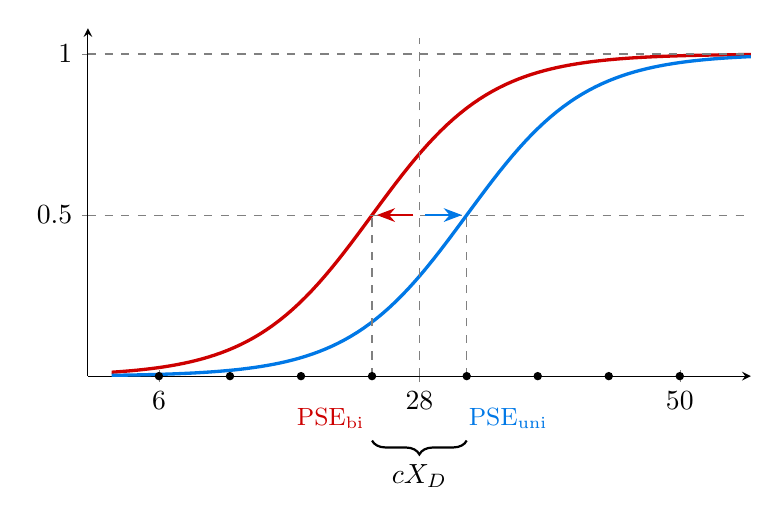
\begin{tikzpicture}
\begin{axis}[width=10cm,height=6cm,
  xmin=0,xmax=56,ymin=0,ymax=1.08,
  xtick={6,28,50},ytick={0.5,1},
  axis lines=left,clip=false]
  \addplot[domain=2:56,samples=100,very thick,bicol]{1/(1+exp(-(x-24)/5))};
  \addplot[domain=2:56,samples=100,very thick,unicol]{1/(1+exp(-(x-32)/5))};
  \addplot[only marks,mark=*,mark size=1.3pt] coordinates{(6,0)(12,0)(18,0)(24,0)(32,0)(38,0)(44,0)(50,0)};
  \draw[dashed,gray] (axis cs:0,1) -- (axis cs:56,1);
  \draw[dashed,gray] (axis cs:0,0.5) -- (axis cs:56,0.5);
  \draw[dashed,gray] (axis cs:28,0) -- (axis cs:28,1.05);
  \draw[dashed,gray] (axis cs:24,0) -- (axis cs:24,0.5);
  \draw[dashed,gray] (axis cs:32,0) -- (axis cs:32,0.5);
  \draw[-{Stealth},thick,bicol] (axis cs:27.5,0.5) -- (axis cs:24.4,0.5);
  \draw[-{Stealth},thick,unicol] (axis cs:28.5,0.5) -- (axis cs:31.6,0.5);
  \node[bicol,font=\small,anchor=north] at (axis cs:20.5,-0.07) {$\PSEbi$};
  \node[unicol,font=\small,anchor=north] at (axis cs:35.5,-0.07) {$\PSEuni$};
  \draw[decorate,decoration={brace,mirror,amplitude=5pt},thick]
    (axis cs:24,-0.2) -- (axis cs:32,-0.2) node[midway,below=5pt] {$cX_D$};
\end{axis}
\end{tikzpicture}
\end{center}

%=====================================================================
\section{Modeling bimanual perceptual interactions in humans}

\subsection{Human 2AFC intensity discrimination task}

M.~Shoaibur Rahman and Jeffrey M.~Yau, \emph{Somatosensory interactions reveal
feature-dependent computations} (Department of Neuroscience, Baylor College of Medicine).

\begin{center}
\timeline{0}{0}
\end{center}
\[
  \operatorname{Prob}[a_c > a_s] = \frac12\left[1+\operatorname{erf}\!\left(\frac{a_c-\mu}{\sigma}\right)\right]
\]
where $a_c$ is the comparison amplitude and $a_s$ the standard amplitude.

\subsection{The distractor reduces the perceived intensity of the standard}

\begin{center}
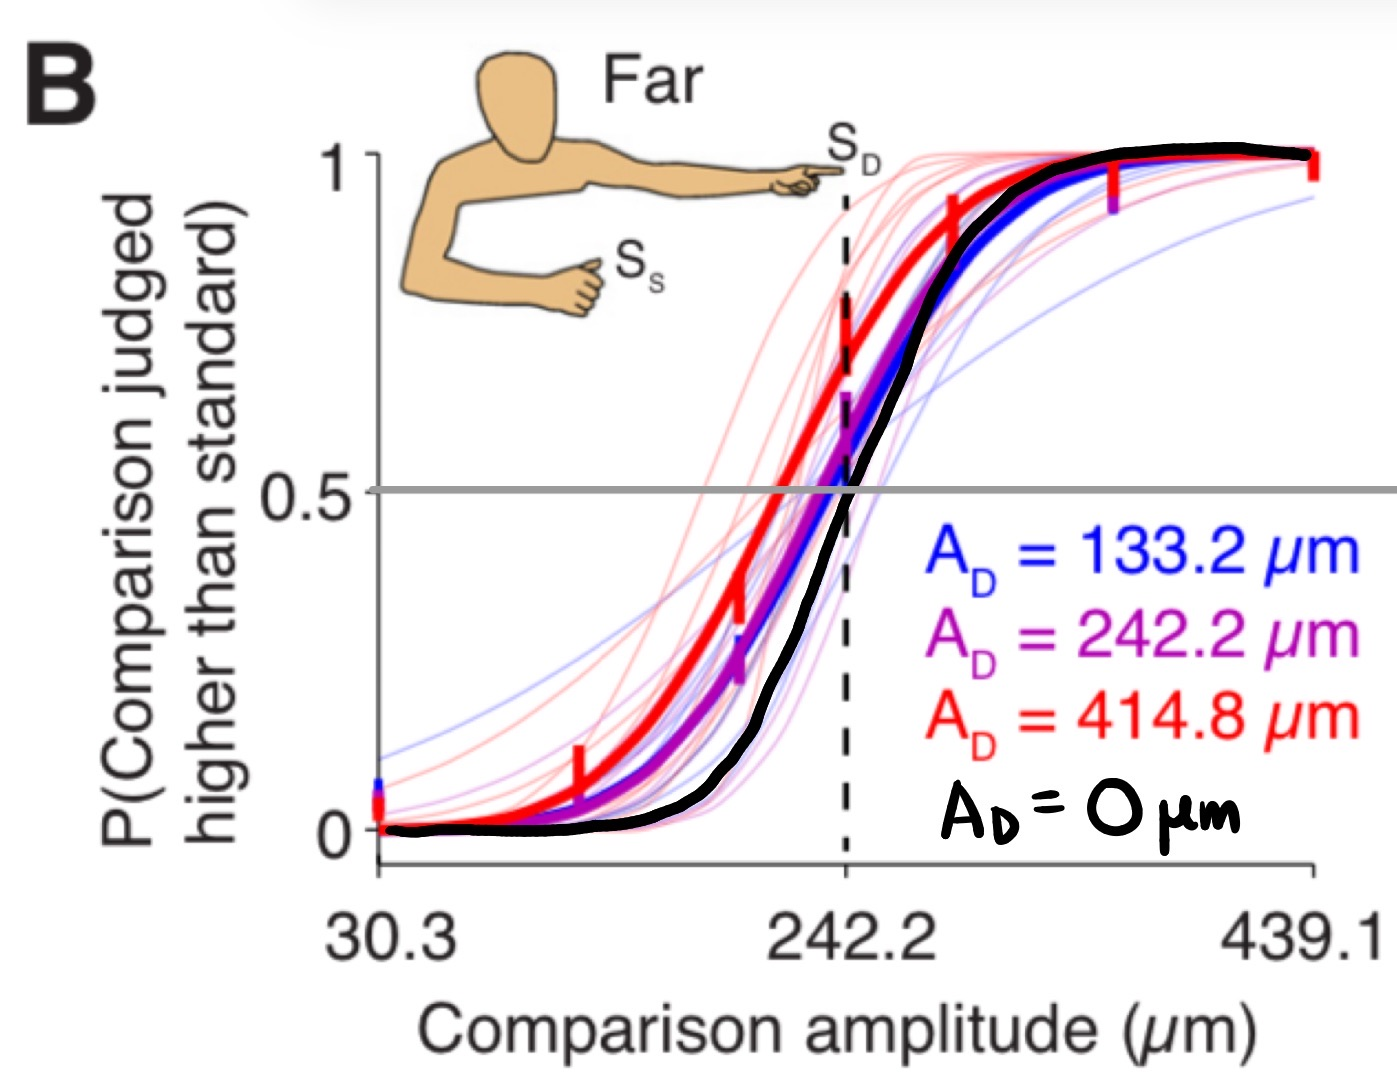
\includegraphics[width=0.6\textwidth]{rahman_yau_fig_annotated.png}
\end{center}
{\small Figure from Rahman \& Yau, panel B; the y-axis is $\operatorname{Prob}[a_c > a_s]$
and the x-axis is $a_c$. The black $A_D = 0\,\mu$m curve was added by hand.}

\begin{itemize}
  \item A stronger distractor gives a greater reduction (curves shift left).
\end{itemize}

\subsection{Modeling}

\textbf{Stimuli:}
\[
  S_S \sim N\bigl[\hat\mu_S, \hat\sigma_S\bigr], \qquad
  S_D \sim N\bigl[\hat\mu_D, \hat\sigma_D\bigr].
\]
\textbf{Final internal estimate of the standard:} ($I$ = truth, i.e.\ the true intensities $I_S$, $I_D$)
\[
  \Theta \sim N[\mu_\Theta, \sigma_\Theta], \qquad
  \underbrace{\mu_\Theta = \frac{I_S}{\alpha + \frac12(I_S + I_D)}}_{\text{divisive normalization}},
  \qquad \sigma_\Theta = \sigma_S .
\]
\textbf{Response probability:}
\begin{align*}
  P[a_c > a_s] = P[a_c > \Theta]
  &= \frac12\left(1+\operatorname{erf}\left[\frac{a_c-\mu_\Theta}{\sigma_\Theta\sqrt2}\right]\right)\\
  &= \frac12\left(1+\operatorname{erf}\left[\frac{1}{\sigma_S\sqrt2}
     \left(a_c - \frac{I_S}{\alpha+\frac12(I_S+I_D)}\right)\right]\right).
\end{align*}

%=====================================================================
\section{Monkey 2AFC intensity discrimination task}

There is no standard stimulus; the distractor is simultaneous with the comparison.
\begin{center}
\timeline{1}{1}
\end{center}
\[
  \operatorname{Prob}[a_c > a_s] = \frac{1}{1+\exp\bigl[-(\beta_0+\beta_1 a_c+\beta_2 I_D)\bigr]}
\]

\subsection{The distractor increases the perceived intensity of the comparison}

\begin{center}
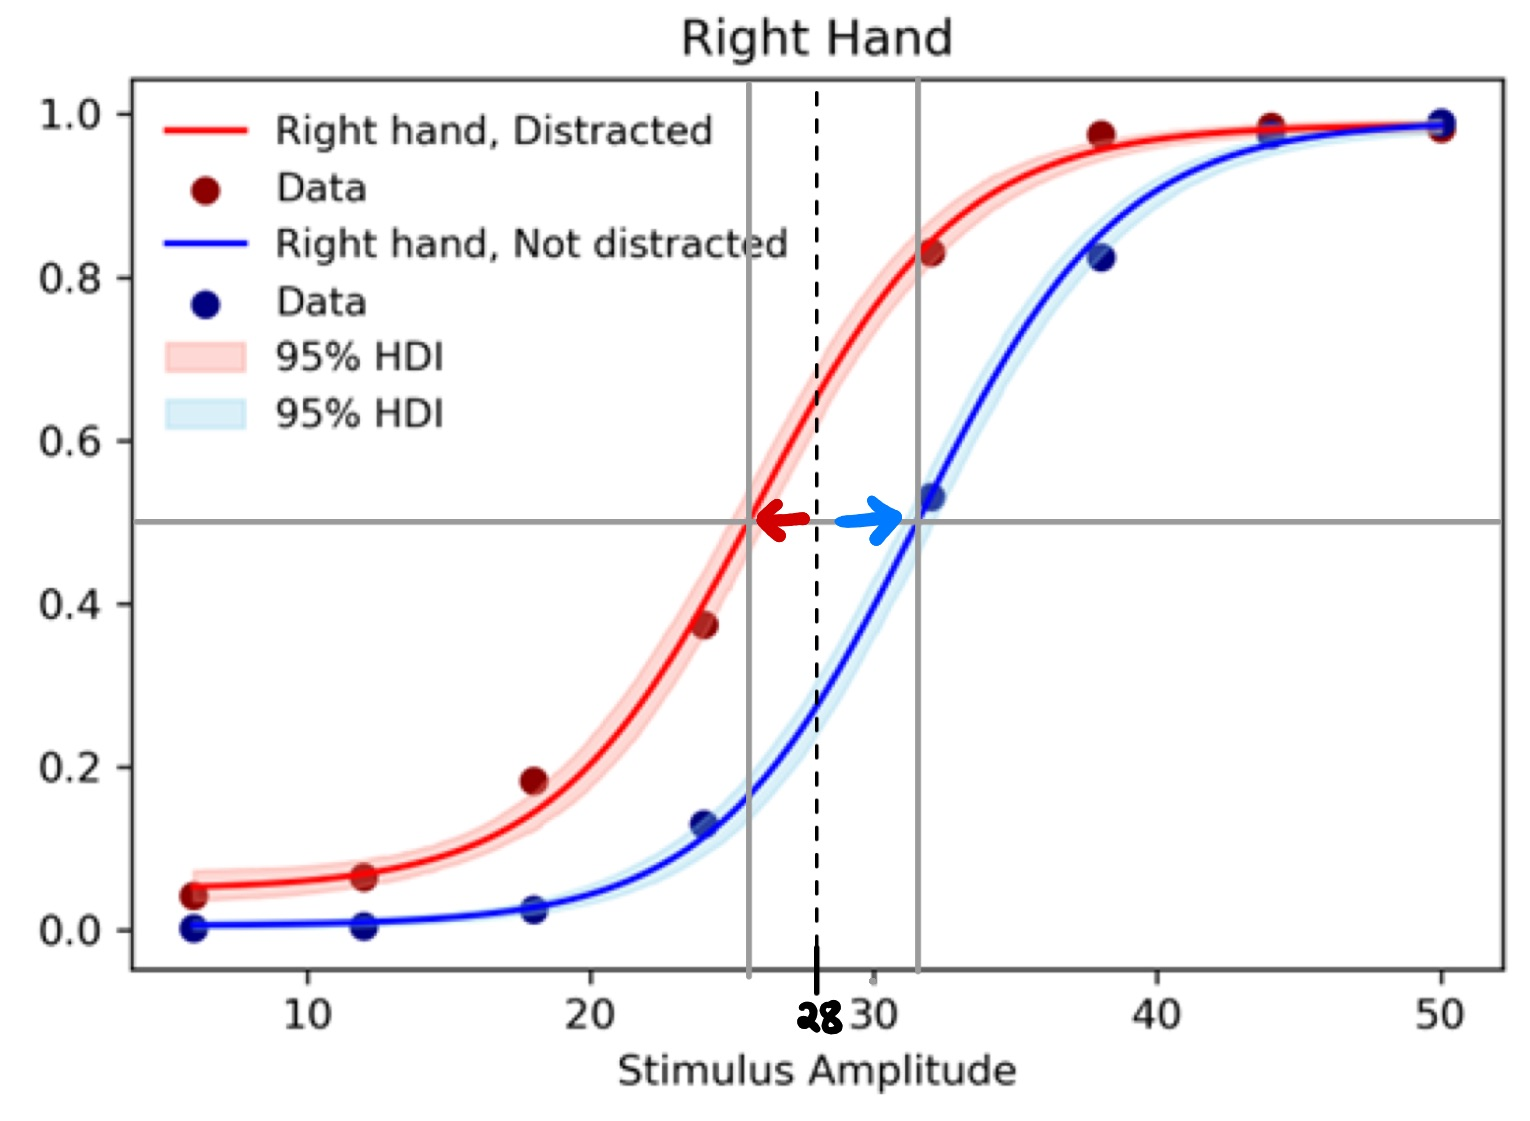
\includegraphics[width=0.6\textwidth]{right_hand_fit.png}
\end{center}
{\small Right hand, distracted vs.\ not distracted, with 95\% HDIs. The y-axis is
$\operatorname{Prob}[a_c > a_s]$, the x-axis (stimulus amplitude) is $a_c$; the middle
dashed line marks 28.}

\begin{itemize}
  \item Equivalently, the absence of a distractor decreases the perceived intensity of
  the comparison stimulus.
\end{itemize}

%=====================================================================
\section{Are the results opposite? Experimental designs}

\begin{center}
\begin{tabular}{p{0.44\textwidth}p{0.44\textwidth}}
\textbf{Humans} & \textbf{Monkeys}\\[2pt]
\begin{itemize}[leftmargin=*,nosep]
  \item no feedback
  \item response = perception
  \item separate unimanual block used for comparison
  \item $\approx 1{,}700$ trials per subject
  \item $30$--$440\,\mu$m
\end{itemize}
&
\begin{itemize}[leftmargin=*,nosep]
  \item correct answers rewarded
  \item response = choice
  \item mixed blocks: unimanual \& bimanual trials
  \item $\approx 17{,}200$ trials per subject
  \item $6$--$50\,\mu$m
\end{itemize}
\end{tabular}
\end{center}

\begin{center}
\scalebox{0.62}{\timeline{0}{0}}\qquad
\scalebox{0.62}{\timeline{1}{1}}
\end{center}

\begin{aside}
Humans: $t$ = standard?
\end{aside}

\begin{center}
\begin{tabular}{p{0.44\textwidth}p{0.44\textwidth}}
\textbf{Humans} & \textbf{Monkeys}\\[2pt]
\begin{itemize}[leftmargin=*,nosep]
  \item receive input
  \item evaluate input
  \item share evaluation
\end{itemize}
&
\begin{itemize}[leftmargin=*,nosep]
  \item receive input
  \item evaluate input
  \item use evaluation to decide what maximizes reward
  \item make choice
\end{itemize}
\end{tabular}
\end{center}

Current monkey model: it is difficult to separate sensory processes from decision strategies.

\begin{tcolorbox}[colback=white,colframe=red!60!black,boxrule=0.6pt]
\textbf{Open question.} Is it possible to construct a model where
\begin{itemize}[nosep]
  \item the structure of $\xp$ makes sense with the attenuation model, and
  \item the decision rule uses $\xp$?
\end{itemize}
\end{tcolorbox}

%=====================================================================
\section{Summary: lab meeting (01/08/26)}

\begin{itemize}
  \item I have a feeling some of our assumptions are wrong, because the human and
  monkey results don't make sense together.
  \item Jeff \& Dr.\ Josi\'c think it still makes sense; it's just the effect of strategy.
\end{itemize}

\subsection*{To ponder}
\begin{itemize}
  \item Why would I set only one threshold instead of using a different one when I
  know I'm being distracted?
  \item Try: extra noise is only present in bimanual trials.
  \item $t$ and $\mu$ are not mutually identifiable, so take $\mu = 0$. Is it OK?
  \item Verify the optimization $t^*$.
  \item Unifying model? Divisive normalization.
\end{itemize}

\subsection*{Next steps}
\begin{itemize}
  \item Prove result.
  \item Code updated for model comparison: pooled; hierarchical additive.
  \item Formulate divisive normalization model: pooled \& hierarchical.
  \item Present Tiny RNN.
\end{itemize}

%=====================================================================
\section{Verifying the optimal threshold $t^*$}\label{sec:verify}

\begin{align*}
  R(t; s, cX_D) = \Biggl[
   &\sum_{i=1}^{4}\frac{1}{1+\exp\bigl[-\frac{1}{s}(t-x_i)\bigr]}
   + \sum_{j=5}^{8}\frac{1}{1+\exp\bigl[\frac{1}{s}(t-x_j)\bigr]}\\
   +&\sum_{i=1}^{4}\frac{1}{1+\exp\bigl[-\frac{1}{s}(t-x_i-cX_D)\bigr]}
   + \sum_{j=5}^{8}\frac{1}{1+\exp\bigl[\frac{1}{s}(t-x_j-cX_D)\bigr]}\Biggr]
\end{align*}
(the constant factor $\frac{1}{16}$ is dropped, since it does not move the maximizer).

\paragraph{Hypothesis.} $t^* \approx 28 + \frac12 cX_D$ maximizes $R(t; s, cX_D)$,
regardless of $s$ and $cX_D$.

\paragraph{Findings} (checked in Wolfram):
\begin{itemize}
  \item $\left.\dfrac{\partial R}{\partial t}\right|_{t=t^*} = 0$ for all $s > 0$ and all $cX_D$. \checkmark
  \item $\left.\dfrac{\partial^2 R}{\partial t^2}\right|_{t=t^*}$ isn't strictly negative. :(
\end{itemize}

\subsection*{Domain considerations}

With $\xp = x_i + cX_D$:
\begin{itemize}
  \item If $x_i + cX_D > t$ for all $i$, the model doesn't make sense, because the
  monkey would only answer \high. So there exists $i$ such that
  $x_i + cX_D < t$, i.e.\ $x_i < t - cX_D$. So $6 < t - cX_D$, i.e.\ $cX_D < t-6$.
  \item If $x_i + cX_D < t$ for all $i$, the model doesn't make sense, because the
  monkey would only answer \low. So there exists $i$ such that
  $x_i + cX_D > t$, i.e.\ $x_i > t - cX_D$. So $50 > t - cX_D$, i.e.\ $cX_D > t-50$.
\end{itemize}
Therefore, for $\left.\dfrac{\partial^2 R}{\partial t^2}\right|_{t=t^*}$ we need only consider
\begin{gather*}
  t^* - 50 < cX_D < t^* - 6\\
  28 + \tfrac12 cX_D - 50 < cX_D < 28 + \tfrac12 cX_D - 6\\
  -22 < \tfrac12 cX_D < 22\\
  -44 < cX_D < 44 .
\end{gather*}

%=====================================================================
\section{Additive models with lapses}

\[
  P[\text{response} = \high] = \gamma_h + (1-\gamma_h-\gamma_\ell)\,
  \frac{1}{1+\exp\bigl(-[\beta_0+\beta_1\xs+\dots]\bigr)}
\]

\begin{enumerate}[label=\Alph*)]
  \item \textbf{Pooled additive model}
  \begin{itemize}[nosep]
    \item partitioned by hand \& distraction status
    \item with lapse parameters
  \end{itemize}
  \item \textbf{Hierarchical additive model}
  \begin{itemize}[nosep]
    \item partitioned by hand \& distraction status
    \item with lapse parameters
    \item partial pooling over sessions
  \end{itemize}
  \item \textbf{Pooled additive model (with distractor)}
  \begin{itemize}[nosep]
    \item distractor amplitude as covariate
    \item partitioned by hand
    \item with lapse parameters
  \end{itemize}
  \item \textbf{Hierarchical additive model (with distractor)}
  \begin{itemize}[nosep]
    \item distractor amplitude as covariate
    \item partitioned by hand
    \item with lapse parameters
    \item partial pooling over sessions
  \end{itemize}
  \item Modify (D) for a linear relationship between the impact of the distractor and
  familiarity with the distractor level.
\end{enumerate}

%=====================================================================
\section{Goals for February--March}

\paragraph{Each additive model:}
\begin{itemize}[nosep]
  \item standardize model structure (necessary for model comparison)
  \item fit model
  \item model recovery
  \item model comparison
\end{itemize}

\paragraph{New model:}
\begin{itemize}[nosep]
  \item formulate divisive normalization model(s)
\end{itemize}

\paragraph{Prove conjecture:} a decision threshold of $t^* = 28 + \frac12 cX_D$ on the
perceived stimulus $\xp = \xs + cX_D + \text{noise}$ maximizes expected reward.

\paragraph{Present} (mention the 1000 neuron competition):
\begin{itemize}
  \item Li Ji-An, Marcus K.~Benna \& Marcelo G.~Mattar, ``Discovering cognitive strategies
  with tiny recurrent neural networks,'' \emph{Nature} \textbf{644}, 993--1001 (2025).
  \item Li Ji-An, ``Tiny recurrent neural networks for discovering cognitive strategies,''
  \emph{Nature Reviews Neuroscience} \textbf{27}, 83 (2026).
\end{itemize}

\end{document}
